\documentclass[\main.tex]{subfiles}

\chapter{Concetualização do Problema}

\section{Requisitos}
Neste capítulo serão definidos os requisitos do projeto. Sejam eles tanto funcionais como não
funcionais.

\subsection{Funcionais}
Representado na figura 3.1, está um \gls{casos de uso} demonstrativo da plataforma de testes
desenvolvida.\par

\begin{figure}[h!]
\centering
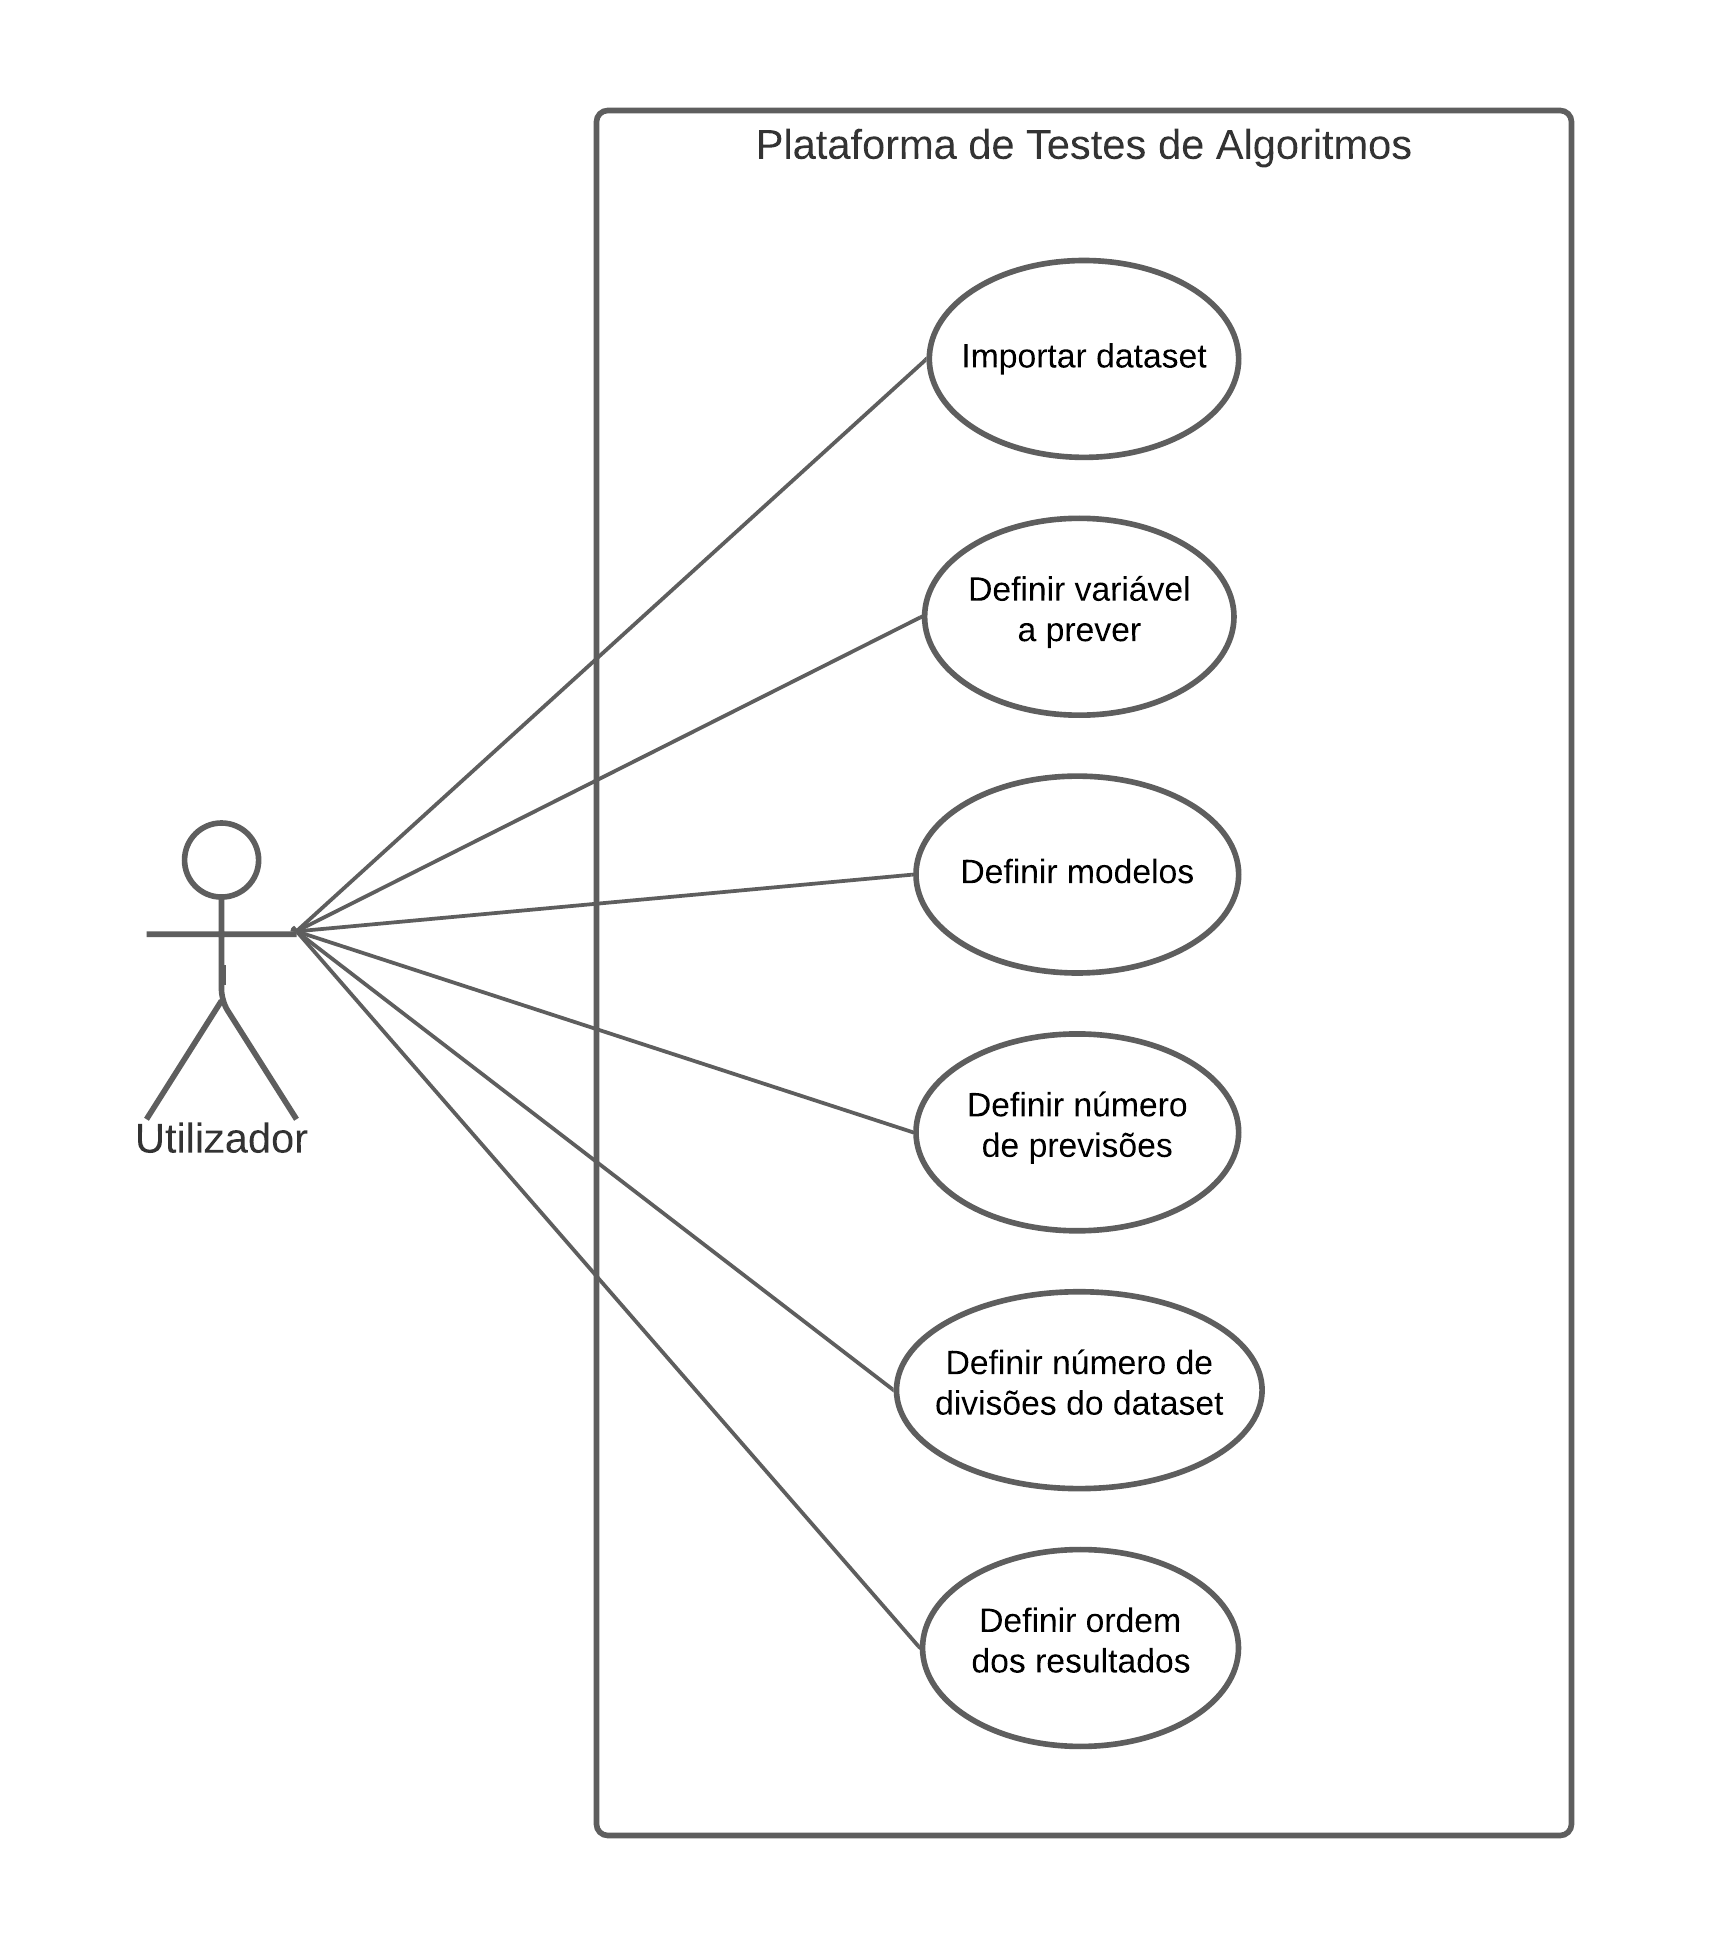
\includegraphics[height=11.5cm]{../private_assets/UseCase_App.png}
\caption{\Gls{casos de uso} da plataforma de testes}
\end{figure}\par

\subsubsection{Carregar dados de \textit{datasets}}
Carregar os dados de um conjunto de dados é um requisito com prioridade alta. Caso seja
necessário, deve ser desenvolvida uma pequena função de tratamento das datas do
\textit{\gls{dataset}}.
Utilizando uma
biblioteca da linguagem \textit{\gls{python}} (\textit{pandas}), temos a capacidade de abrir
um ficheiro \textit{.csv} e carregá-lo para um objeto \say{\textit{DataFrame}}. Deste objeto,
pode ser retirada a informação desejada do conjunto de dados ou até mesmo exportar um gráfico
com os seus dados.

\subsubsection{Dividir em \textit{datasets} de treino e de teste}
Em primeiro lugar, o utilizador deve introduzir o número de vezes que o dataset deve ser
dividido, caso seja pretendido realizar validação cruzada nos testes dos modelos. Se não
for introduzido nenhum valor, é subentendido que não será para utilizar esta técnica na
realização dos testes.\par
Após carregar os dados do \textit{\gls{dataset}} os dados são separados em dados de treino e 
dados de teste. A quantidade de dados de teste pode ser definida pelo utilizador através de
dois parâmetros (através da percentagem do dataset de teste ou através do número de
previsões a realizar - caso seja introduzida uma percentagem do dataset de teste, o número
de previsões é calculado a partir desse valor e é ignorado o número introduzido pelo
utilizador).

\subsubsection{Executar vários algorimos ao mesmo tempo}
Este é talvez o requisito mais importante e mais meticuloso de todo o projeto. É essencial
que o estudo dos modelos (\textit{\acrshort{arima}}, \textit{\acrshort{arimax}},
\textit{\acrshort{sarima}} e \textit{\acrshort{sarimax}}) seja bem feito e que exista uma boa
compreensão dos mesmo também, caso contrário, não só a teoria do projeto fica mal entendida,
como o projeto em si fica prejudicado pelo mau desenvolvimento da plataforma\cite{numerical_methods}.\par
Para realizar a execução dos modelos, o utilizador deve indicar os algoritmos que pretende
testar e os parâmetros comuns e não comuns de cada algoritmo.

\subsubsection{Guardar dados de previsões bem sucedidas}
Após a conclusão de cada modelo, caso tenha terminado com sucesso, deve ser exportado um
ficheiro \textit{.csv} com as previsões e dados de teste para dentro da pasta de cada modelo,
que, por sua vez, se encontrará localizada na pasta global dos resultados.

\subsubsection{Guardar gráficos de previsões bem sucedidas}
Após a conclusão de cada modelo, caso tenha terminado com sucesso, deve ser exportado uma
imagem (\textit{.png}) com o gráfico das previsões do modelo. Tudo isto será exportado para
dentro da pasta de cada modelo, que, por sua vez, se encontrará localizada na pasta global
dos resultados.

\subsubsection{Exportar ficheiro com sumário dos resultados de todos os modelos}
No final, quando todos os modelos tiverem terminado, será exportado para a pasta global dos
resultados um ficheiro \textit{.csv} com uma avaliação de todos os modelos. Estes serão
ordenados por um parâmetro definido pelo utilizador, podendo ser uma ordem por Tempo de
Execução, \acrlong{mae} (Mean Absolute Error - \acrshort{mae}), \acrlong{mse} (Mean
Squared Error - \acrshort{mse}) ou \acrlong{rmse} (Root Mean Squared Error - \acrshort{rmse}).

\subsubsection{Exportar ficheiro com o registo da execução de cada modelo}
No final, quando todos os modelos tiverem terminado, será exportado para a pasta global dos
resultados um ficheiro \say{\textit{log.txt}} com a visão geral de cada modelo.


\subsection{Não Funcionais}

\subsubsection{Continuar aplicação no caso da falha de algum modelo}
A aplicação deve manter-se estável e sem qualquer tipo de problema caso algum dos modelos
falhe. Nestes casos, a situação é reportada para o ficheiro de registos e no fim exportada
com os resultados de todos os modelos.

\subsubsection{Guardar dados de forma persistente}
Os dados de cada modelo são guardados de forma persistente, isto é, mesmo que a aplicação
seja encerrada manualmente, as previsões e os gráficos gerados até ao momento nunca serão
perdidos. Este requisito é bastante importante neste tipo de projetos, visto que grande
parte dos modelos falham ou por vezes não deixam a aplicação terminar, o que obriga a
forçar o término da mesmo. No entanto, os dados dos modelos testados até ao momento
permanecem intactos.

\subsubsection{Adaptar \textit{scripts} para correr em ambiente do \textit{Google Colab}}
Depois da plataforma de testes estar realizada, para finalizar, é necessário fazer a
integração com o \textit{\gls{google colab}}, que é uma suíte de computação gratuita,
oferecida pela \textit{\gls{google}}. Feito isto, devem ser realizados alguns testes para
comprovar a funcionalidade do projeto na plataforma desejada.

\newpage